
One other goal of the thesis is to evaluate the recognition performance based on a number of connected LMC sensors and test the capabilities of \nameref{ch:multileap} library in the real-time environment using various layouts with a different number of sensors. Results from one connected sensor served as the reference, mostly whether having multiple LMC sensors does improve the recognition of difficult angles or not. We also examined how effective was MultiLeap's merging for gestures presented in simple default angles.

We used the demo application and trained model as described in section \ref{real_time_recognition}. The model was trained on our original dataset from section \ref{data_sampling}. 

\section{Testing Method}

For each gesture, we performed 1000 classifications. We did not exclude classifications with corrupt sequences, such as when the LMC sensor did not get a correct hand skeletal alignment of the presented hand. We wanted to emulate genuine user interaction with the LMC. Each gesture was held in various positions and angles in a certain span of time until the number of classification was not satisfied. 

Results of multiple LMC sensors are an average of 5 different automatic calibrations. There is currently no telling how well sensors were calibrated. Therefore, we want to avoid generalizing MultiLeap capabilities base on experiments conducted on only one calibration. An experimental feature is being currently worked on to recognize the calibration quality, but it was not dependable enough in the time of our experiments.

Dynamic gestures were not tested, as it is hard to evaluate the percentage of correct classifications in a continuous stream of data. If we test dynamic gestures without any mix-up with static gestures, it will defeat the purpose of testing in a real-time environment. We want to evaluate the performance when a dynamic gesture is performed in the middle of the sequence of static gestures, as to whether the trained model is capable of recognizing the difference between the static gesture of \textit{number 5} as oppose to having \textit{number 5} moving quickly to one side, doing a \textit{swipe}. Despite not dedicating any experiments to dynamic gestures, we can still evaluate responsiveness and general correctness when we perform it. We also want to keep track of times when a static gesture gets misclassified for a dynamic gesture, and what is the percentage of valid classification to determine whether the threshold for prediction probability was not set too high.


\subsection{One Leap Motion Sensor}

Experiments for a single connected sensor were performed with LMC's VRVisualizer to understand better how the skeletal structure, which gets classified, looks. It helps us distinguish whether misclassification is caused by our trained model or by LMC's hand joint misalignment.

\begin{figure}[ht]
    \centering
    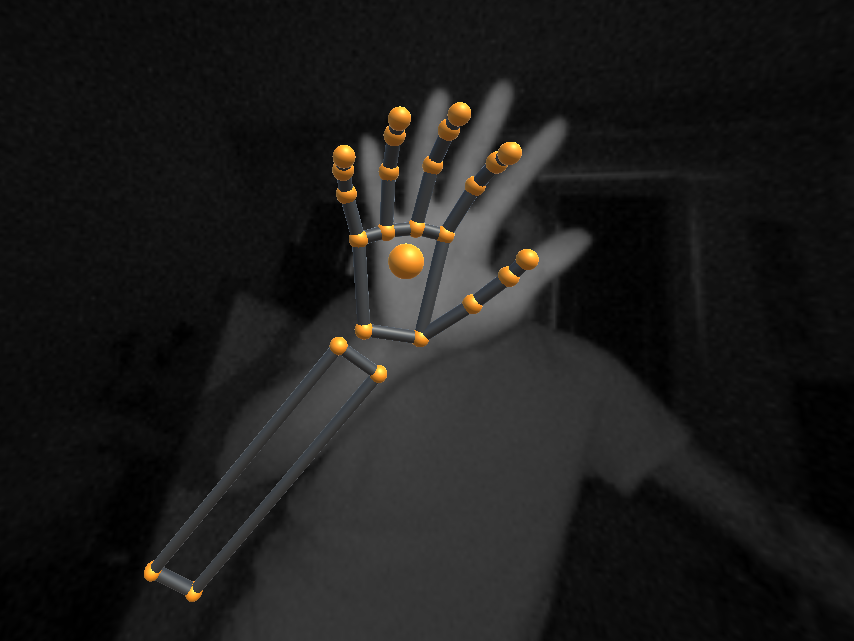
\includegraphics[width=7cm]{vrvisualizer.png}
    \caption{VRVisualizer}
    \label{fig:vrvisualizer}
\end{figure}

\begin{figure}[ht]
    \centering
    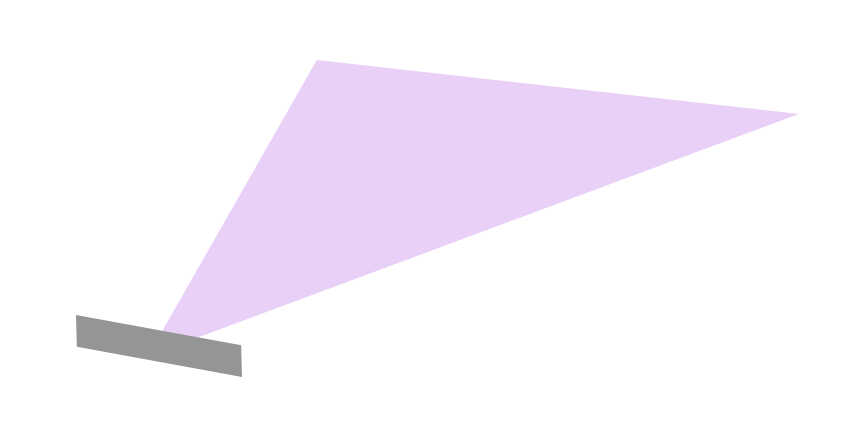
\includegraphics[width=7cm]{setup_1.png}
    \caption{Ilustrative field of view of 1 LMC sensor}
    \label{fig:setup_1}
\end{figure}


The classification was responsive with every presented gesture, including dynamic gestures. Still, the limitation of having only one sensor presents itself when we perform a gesture of \textit{number 1} pointing towards the sensor. The sensor struggles to recognize the pointing finger as being straight, and often times it misclassifies the gesture as a fist, or the prediction does not meet the threshold requirement. It also struggles with the prediction of \textit{number 3} and \textit{number 4}, wherein various angles, the thumb is not recognized by LMC as bent and straighten correctly. Gestures then get confused with \textit{number 2}, and \textit{number 5} respectively. The \textit{pinch} gesture was mostly misclassified due to hand joint misalignment by the LMC sensor. We could be questioning the trained model's performance due to training on a not optimal dataset, but when the hand joint was aligned correctly, the gestures also got classified correctly without any further complications.

The percentage of invalidated gestures was also not too high as most of the discarded predictions were of 0.8 probability and lower. We can assume that our set threshold of 0.9 is not overly strict for the prediction.

\begin{figure}[ht]
    \centering
    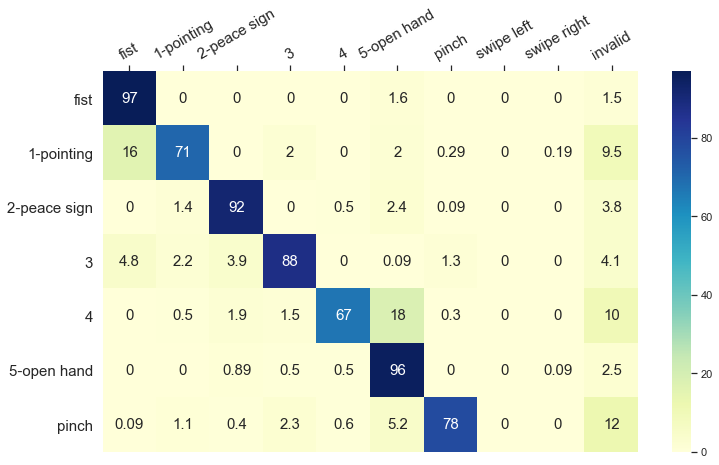
\includegraphics[width=12cm]{one_leap.png}
    \caption{Confusion matrix of prediction by using 1 LMC sensor}
    \label{fig:confuse_1}
\end{figure}


\subsection{Two Leap Motion Sensors}

For two sensors, we explored several layouts with different calibrations. We could not utilize VRVisualizer as we did with one LMC sensor. The MultiLeap library does not have a feature of visualizing the merged hand or any visualization during calibration at the moment. Therefore, we could not accurately evaluate how the merged hand structure looks like during classification or calibration. Thus, our experiments are limited in correction when evaluating the accuracy of multiple LMC sensors. We recommend conducting experiments again once the visualizing feature is implemented.

\subsubsection{Parallel Layout}
\label{parallel_layout}

The parallel layout, with sensors facing each other, could not be tested. LMC sensors expect to receive its emitted IR signals to return from a hand. Instead, the emitted IR signal is received by the other sensor and vice versa. The behavior will confuse LMC recognition making the sensors think there is a hand presented even when it is not. Thus we assume this parallel layout is inappropriate to be a part of any setup with multiple LMC sensors.

\begin{figure}[H]
    \centering
    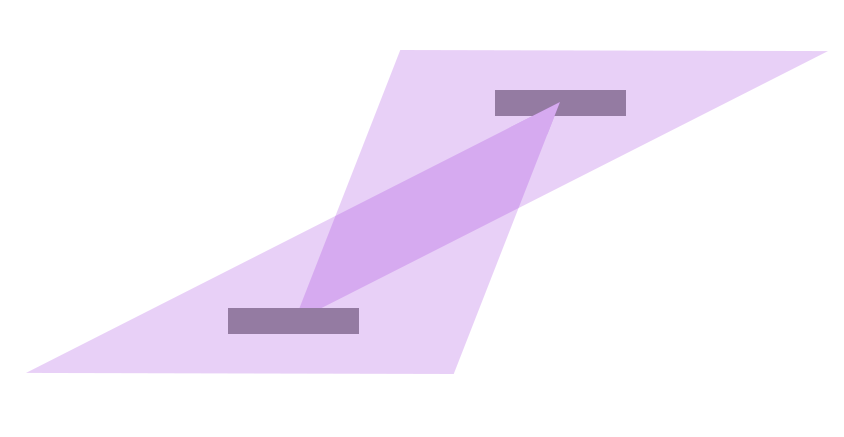
\includegraphics[width=7cm]{setup_2_para.png}
    \caption{Parallel placement layout for 2 LMC sensors}
    \label{fig:setup_2_para}
\end{figure}

\subsubsection{Non-parallel Layout}

Sensors were placed next to each other at a slight angle facing inwards, avoiding sensors to be disturbed by other's emitted IR signals.

\begin{figure}[ht]
    \centering
    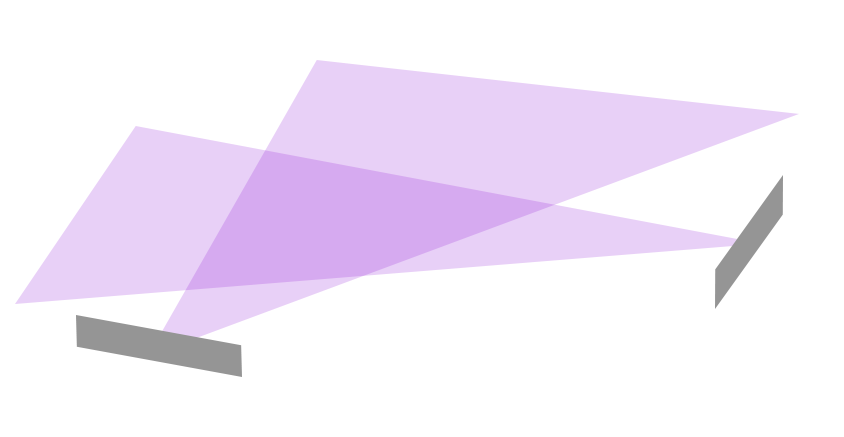
\includegraphics[width=7cm]{setup_2_non.png}
    \caption{Non-parallel placement layout for 2 LMC sensors}
    \label{fig:setup_2_non}
\end{figure}

Using MultiLeap \cite{tomasMultileap} showed improvements in classifying gestures in difficult angles, which it struggled in previous experiments with one connected sensor. The MultiLeap was able to capitalize on the advantage of having multiple fields of view for capturing a presented hand.

Despite improved performance with various angles, the number of invalidated classifications had increased. The average prediction probability for gesture was 0.697, which is most likely caused by misalignment when merging hands. The number of confusion between gestures had also increased. Both could be caused by poor calibration, which there is currently no way to identify the calibration quality in order to avoid this issue. 

\begin{figure}[ht]
    \centering
    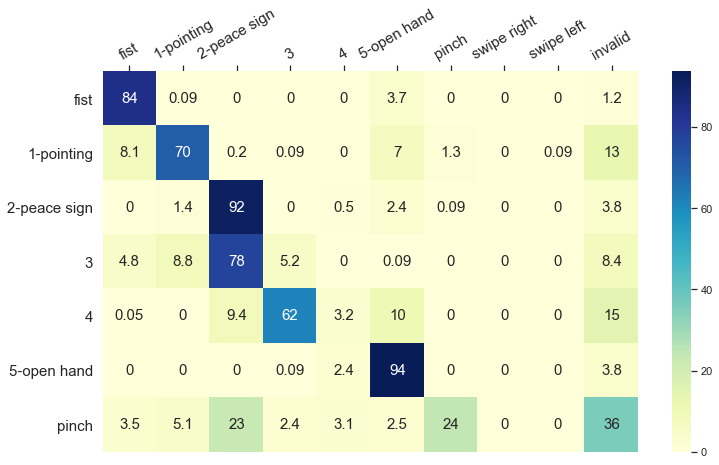
\includegraphics[width=12cm]{two_leap.png}
    \caption{Confusion matrix of prediction by using 2 LMC sensors}
    \label{fig:confuse_2}
\end{figure}

The calibration quality significantly affects the prediction accuracy. More specifically, when we tested \textit{pinch} gesture, the measured average accuracy was mere 24.4\%, but when tested again with a new calibration, the accuracy improved up to 83\%, which is already better than referential results of one connected sensor. The calibration could also affect dynamic gestures. While performing experiments, dynamic gestures were not responsive as they were with only one connected sensor. Often times they were not recognized at all, but their responsiveness varied with different calibrations. 

The MultiLeap's current most notable issue is an incorrect number of reported hands. Our demo application does not make a prediction when there is more than one hand presented. This feature is conflicting with the current bug of MultiLeap, where it frequently returns two hands instead of one, even though only one is present, which from a user's point of view makes the demo application almost unusable for any accurate consecutive recognition. However, the issue is known, and its fix is currently in development.

\subsection{Three Leap Motion Sensors}

Sensors were carefully placed into a triangular layout so that LMC sensors don't emit IR signals to others, recreating a similar misrecognition issue as in section \ref{parallel_layout}.

\begin{figure}[ht]
    \centering
    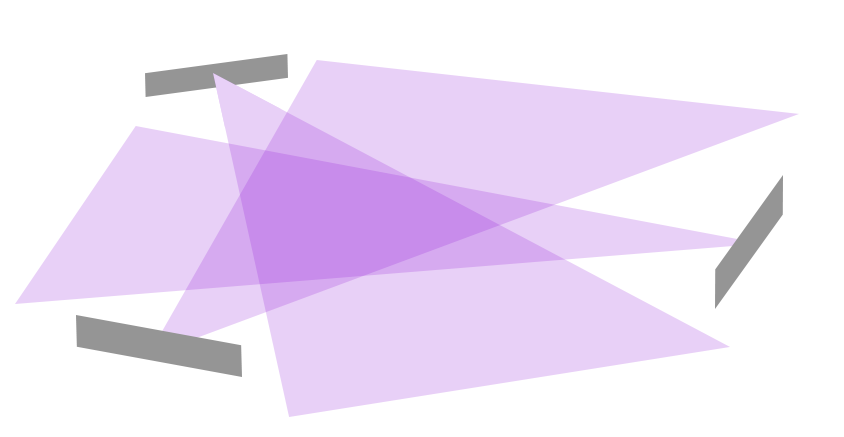
\includegraphics[width=7cm]{setup_3.png}
    \caption{Placement layout for 3 LMC sensors}
    \label{fig:setup_3}
\end{figure}


Using three sensors shares similar behavior as using two sensors. The improvement in recognition of difficult angles was improved upon additional sensors in fewer cases of calibration. Most of the calibrations made did not capitalize properly on the advantage of having multiple sensors. 

The setup suffered similarly, if not at times more, on the side of increased invalidated classification. The average prediction probability for gesture was 0.6841. The issue with the incorrect number of reported hands still persists in a similar frequency as it did with two connected sensors.

\begin{figure}[ht]
    \centering
    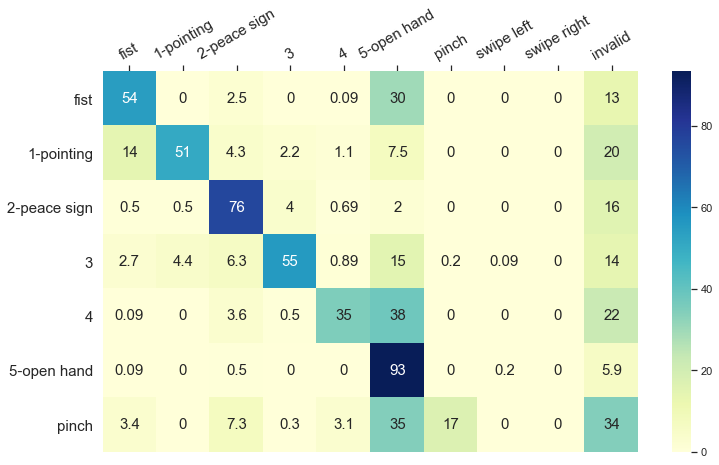
\includegraphics[width=12cm]{three_leap.png}
    \caption{Confusion matrix of prediction by using 3 LMC sensors}
    \label{fig:confuse_3}
\end{figure}

The \textit{pinch} alongside with \textit{number 4} gesture has low accuracy across all 5 different calibrations. They often got confused with the gesture of \textit{number 5}. Dynamic gestures also suffered where the responsiveness seemingly did not change with various calibrations. We can only assume that having more sensors is harder to calibrate and more demanding on calibration quality.



